% !TeX encoding = utf8
%\documentclass[conference]{IEEEtran}
\documentclass[conference,10pt,a4paper]{IEEEtran}  
\IEEEoverridecommandlockouts
% The preceding line is only needed to identify funding in the first footnote. If that is unneeded, please comment it out.
%\pdfminorversion=7
\usepackage{stfloats} 
\usepackage{amsmath,amssymb,amsfonts}
\usepackage{algorithmic}
\usepackage{graphicx}
\usepackage{textcomp}
\usepackage{xcolor} 
\usepackage{cancel}


%\usepackage{helvet}
%\usepackage{tikz}
%\usepackage[scaled]{uarial}

\renewcommand*\familydefault{\sfdefault}

\usepackage[T1]{fontenc}
\usepackage[utf8]{inputenc}




\definecolor{color1}{RGB}{200,200,200}

\usepackage[hidelinks 	= 	true, 
draft 		=	false,	% all hypertext options are turned off
final 		=	true, 	% all hypertext options are turned on
raiselinks 	= 	true,	% Allow links to reflect real height - e.g. with pictures
breaklinks	=	false,	% false=Do not break a line within a link
backref		=	false,	% false=no backlinks in the bibliography
pagebackref =	false,	% false=no pagebacklinks in bibliography
linktocpage =	true,	% true=makes page-no linked and not text in TOC,LOF and LOT
%			colorlinks	=	true,	% true=Colors the text of links and anchors
colorlinks	=	false,	% true=Colors the text of links and anchors
%			linkcolor 	=	red, 	% Color for normal internal links.
%			anchorcolor =	black, 	% Color for anchor text.
%			citecolor 	=	green, 	% Color for bibliographical citations in text.
%			filecolor 	=	cyan, 	% Color for URLs which open local files.
%			menucolor 	=	red,	% Color for Acrobat menu items.
%			runcolor 	= filecolor,% Color for run links (launch annotations).
%			allcolors 	= 	red,	% Set all color options (without border and field options).
allcolors   =   color1, 
urlcolor 	=	color1,	% Color for linked URLs.
allbordercolors  =color1,	% Set all colors
%			citebordercolor =green,	% cite color
%			filebordercolor =cyan,	% file color
%			linkbordercolor =red,	% link color
%			urlbordercolor  =blue,	% url color
%			pdfborder 			= 0 0 0,% weder farbige links noch umrandung			
%			menubordercolor 	= red,	% set menu color
%			frenchlinks 		= false,% Use small caps instead of color for links.
bookmarks			= true,	% true=Bookmarks are added to the pdf
bookmarksopen 		= false,% false=Bookmarks not open when opening the pdf
bookmarksnumbered 	= true,	% true= Eintraege sind nummeriert 
%			pdfpagemode	=	FullScreen,	% File is opened in Full Screen
%			pdfstartview=	fit,	% Fit size when opening pdf
pdfpagelabels=	true,	% true = Roemische Zahlen usw werden dargestellt,
% false= fortlaufende nummerierung
]{hyperref}
 
 

 
 
% \title{Charakterisierung einer Schraubenverbindung mittels magnetischem Sensor-Array}
%\title{Characterization of a Bolted Joint with a Magnetic Sensor Array}
%\title{Magnetic Sensor Array for Determination of the Applied Preload of a Bolted Joint}
\title{\fontsize{16pt}{18pt}\selectfont\bfseries Histogramm-Verfahren für die Signalaussteuerung bei der Impedanzspektroskopie für Fahrzeugbatterien\\[12pt]
	\fontsize{10pt}{11.5pt}\selectfont\normalfont\itshape
	$\underline{\text{Tobias Frahm}}$ , 
		Florian Rittweger, Thorben Schüthe, Karl-Ragmar Riemschneider \\~\\
 Hochschule für Angewandte Wissenschaften Hamburg, Berliner Tor 7, 20099 Hamburg \\
 
	
}
 

 

\usepackage{booktabs}
\usepackage{multirow} 
\usepackage{amsmath}
\usepackage{siunitx} 
\sisetup{locale = DE,  
	separate-uncertainty,  
	%	range-units = brackets,  
	range-units= repeat, 
	range-phrase= ~bis~ ,
	list-units = single,  
	%	per-mode=symbol,
	per-mode=symbol-or-fraction,
	round-precision=3}

\DeclareSIUnit\Nm{Nm}
\DeclareSIUnit\Nm{Nm}
\usepackage[left=2.5cm,right=2.5cm,top=2.5cm,bottom=2.5cm]{geometry}

\usepackage{mathtools}
\usepackage{xspace}
%\usepackage{tools-overview}


\usepackage[main=ngerman]{babel} 
\usepackage[babel]{csquotes} 
%\usepackage[]{caption} 
%\captionsetup{format=} 
\usepackage[figurename=Abb.,
			tablename=Tab.,
			format=hang,
			textfont=it,
			labelfont=it,
			labelsep=quad,
			skip=1em]{caption}  
%\setlength{\belowcaptionskip}{-1em}



%\usepackage[%
%style		= ieee,    
%defernumbers= true,      % to set different numeric types -e.g. A1...A2 B1...B2
%sortcase	= false,%		% false- keine unterscheidung zwischen gross und kleinschrift 
%bibencoding	= utf8,%
%doi 		= true, 
%isbn 		= false,
%subentry	= false,
%url 		= false,  
%backend		= biber,
%language    = {ngerman},
%maxcitenames=2,
%mincitenames=2,
%]{biblatex}				% um 8-bit zeichen zu erkennen, fuer umlaute 

%\DeclareFieldFormat{url}{Available\addcolon\space\url{#1}}
%\DefineBibliographyStrings{german}{
%	andothers = {{et\,al\adddot}},
%	and = \&,
%	page = {\:}
%} 
%\addto\extrasenglish{\languageshorthands{ngerman}} 
\usepackage{upgreek}
\usepackage{ltablex}
\bibliography{Bibliography/lit.bib}	 
  

%\DefineBibliographyStrings{english}{andothers = \mkbibemph{et al\adddot}}
%\DefineBibliographyStrings{german}{andothers = \mkbibemph{et al\adddot}}
 
% \newcommand*\circled[1]{\tikz[baseline=(char.base)]{
% 		\node[shape=circle,draw,inner sep=2pt] (char) {#1};}}
\setlength{\columnsep}{10mm} 
\renewcommand{\IEEEkeywords}{\textbf{Keywords:}}
\renewcommand{\abstract}{{\fontsize{12pt}{10pt}\selectfont\bfseries Zusammenfassung}\\[.5em]}

\makeatletter
\renewcommand\section{\@startsection {section}{1}{\z@}%
	{-3.5ex \@plus -1ex \@minus -.2ex}%
	{3pt \@plus.2ex}%
	{\normalfont\bfseries}}
\makeatother

\def\thesection{\arabic{section}}
\usepackage{titlesec}
%\titleformat{\section}{\normalfont\bfseries}{\thesection}{1em}{}
\titlespacing*{\section}{0em}{6pt}{3pt}

%\makeatletter
%\renewcommand\paragraph{\@startsection{paragraph}{4}{\z@}%
%	{1em \@plus1ex \@minus.2ex}%
%	{-1em}%
%	{\bfseries\normalsize}}
%\makeatother



\setlength{\parindent}{0pt}
%\usepackage[none]{hyphenat}
%\geometry{showframe}
\usepackage{layouts}
\usepackage{float}
%\usepackage{newtxtext}
\usepackage{pifont}
\usepackage{nicematrix}
\usepackage{tikz}
\usetikzlibrary{positioning}


\newcommand{\matrixA}{% 
	$\begin{bNiceMatrix}
		k_{1,1,1}& \Cdots        & k_{v,1,1}\\
		\Vdots      	& \Ddots     	&  \\
		k_{1,k,1} &               & k_{v,k,1}\\
	\end{bNiceMatrix}$
}   

\newcommand{\matrixB}{% 
	$\begin{bNiceMatrix}
		k_{1,1,c} & \Cdots        &k_{v,1,c}\\
		\Vdots          &\Ddots         & \\
		k_{1,k,c} &               &k_{v,k,c}\\
	\end{bNiceMatrix}$
} 

\newcommand{\matrixC}{% 
	$\begin{bNiceMatrix}
		k_{1,1,1} & \Cdots        & k_{v,1,1}\\
		\Vdots      	& \Ddots     	&  \\
		k_{1,k,1} &               & k_{v,k,1}\\
	\end{bNiceMatrix}$
}

\newcommand{\matrixD}{% 
	$\begin{bNiceMatrix}
		k_{1,1,1} & \Cdots        & k_{v,1,1}\\
		\Vdots      	& \Ddots     	&  \\
		k_{1,k,1} &               & k_{v,k,1}\\
	\end{bNiceMatrix}$
}


\DeclareCaptionLabelSeparator{colonquad}{:\quad}
\SetCaptionDefault{labelseparator}{colonquad}
\begin{document}  
	\def\X#1{% 
		\ding{\numexpr171+#1\relax}%
	}
%	\maketitle    
	\twocolumn[
	\begin{@twocolumnfalse}
		\vspace*{.3cm}
%		\vspace*{1.02cm}
		\maketitle 
	\end{@twocolumnfalse}
	\vspace*{-1.4cm}
	\begin{abstract}
		\fontsize{10pt}{12pt}\selectfont
		Die bewährte Methode der Elektrochemischen Impedanzspektroskopie soll in Zukunft auf das gesamte Energiespeichersystem in Elektrofahrzeugen angewandt werden.
		Die erfassten Spannungsantworten der Batteriezellen weisen besonders kleine Amplituden und schlechte Störabstände auf. In diesem Kontext soll ein messtechnisches Teilproblem untersucht werden. Für die Umsetzung war es Aufgabe, durch einen steuerbaren Vorverstärker den Dynamikbereich des Analog-Digital-Wandlers (ADC) maximal auszunutzen. Aufgrund der schlechten Signalqualität bei hoher Verstärkung führt das zu frühzeitiger Übersteuerung des ADC. Hieraus ergaben sich zwei Zielstellungen. Zum Einen war die Sättigung des ADC zu erkennen und in der Signalauswertung zu berücksichtigen. Zum Anderen sollte der durch Sättigung entstehende Fehler bestmöglich kompensiert werden. Als Randbedingung musste sich auf Methoden beschränkt werden, welche mit minimalem Rechenaufwand im Sensorchip für jede Batteriezelle implementiert werden können. 
    	Der Lösungsansatz greift auf die fortlaufende Beobachtung des abgetasteten Signals mit einfachen statistischen Verfahren zurück. Es werden dabei drei Parameter ermittelt: der Anteil der Datenpunkte in Sättigung, die Varianz und Kurtosis der verbleibenden Datenpunkte, die sich nicht in Sättigung befinden. Es kann einen Zusammenhang dieser Größen mit der Signalamplitude ermittelt werden. Dieser kann zur Steuerung des Vorverstärkers herangezogen werden, um die Übersteuerung zu reduzieren. Alternativ kann ein Korrekturfaktor errechnet werden, welcher die fehlerhaft ermittelte Signalamplitude weitgehend ausgleicht. Dieser Korrekturfaktor kann bei der Berechnung der Impedanz eingesetzt werden. Die vorgestellten Ergebnisse zeigen, dass damit die negativen Auswirkung für das zu bestimmende Impedanzspektrum infolge der Übersteuerung deutlich zu reduzieren sind.
	\end{abstract}
	\vspace{.5em}
	\begin{IEEEkeywords}
		\fontsize{10pt}{12pt}\selectfont
		\normalfont Elektrochemische Impedanzspektroskopie, Mixed-Signal-Processing, Histogramm, ADC-Clipping
	\end{IEEEkeywords} 
	\vspace{3em}
	] 
	%===============================================================
	% 	Einleitung 
	%===============================================================
\graphicspath{{./BILDER}}
\section{Einleitung}	

In Elektrofahrzeugen der nächsten Generation soll auch das Batterie-Management-System (BMS) verbessert werden. Zu diesem Zweck gibt es das Bestreben, die im Labor etablierte Methode der Elektrochemischen Impedanzspektroskopie (EIS) einzusetzen. Mithilfe der EIS lassen sich wertvolle Informationen über den Zustand der Batteriezelle ableiten, hierzu gehören der aktuelle Ladezustand, die Zellalterung, die Leistungsprädiktion und die Innentemperatur [4]. Im Fahrzeug werden die Batteriezellen mit niederfrequenten Wechselströmen angeregt, die an jeder Batteriezelle eine Spannungsantwort erzeugen [3]. Aus dem Wechselstrom und der Spannungsantwort wird die Impedanz für ein Spektrum von Anregungsfrequenzen errechnet. In Elektrofahrzeugen werden niederohmige Batteriezellen (typisch: $R_i < \SI{1}{m\Omega}$) eingesetzt werden. Zudem ist der Anregestrom aus Gründen der verfügbaren Energie und des Schaltungsaufwands limitiert. Für die Wechselströme zur Anregung wird eingeschätzt, dass der Bereich zwischen $\SI{1}{A}$ und $\SI{10}{A}$ umsetzbar ist. Infolgedessen liegen die Spannungsantworten in der Größenordnung  von $\SI{1}{mV}$. Sie sind mindestens prozentgenau, d.h. auf sieben Bit oder mehr digital aufzulösen. Die Messsysteme hierfür benötigen analoge Verstärker. Zudem muss eine Subtraktion des Gleichanteils der Zellspannung erfolgen. Dies kann durch eine steuerbare Subtrahiererschaltung oder eine kapazitive Wechselstromkopplung erfolgen. Letzteres ist für niederfrequente Anregung bis unter ein Hertz nicht mehr technisch umsetzbar, weil die notwendigen Kondensatoren sehr groß würden. Daher wird der Gleichanteil auch durch eine steuerbare Referenzspannung kompensiert. Diese wird ebenfalls vom erfassten Digitalsignal errechnet. Dabei wird eine symmetrische Nutzung des Dynamikbereichs des ADC angestrebt. 
Weil Verstärkungsfaktoren in der Größenordnung von $1000$ mitunter erforderlich sind, unter Praxisbedingungen werde typisch starke Stör- und Rauscheinflüssen auftreten. Die Verstärkungsfaktoren sind nur begrenzten Anzahl an Stufen einstellbar. In der Gesamtheit führt das zu einem Widerspruch bei der Auslegung der analogen Vorverarbeitung. Entweder wird auf Signalauflösung verzichtet oder es wird ein Fehler durch teilweise Übersteuerung unvermeidbar. Dieser Gegensatz ist der Ausgangspunkt für den nachfolgend vorgestellten Lösungsansatz.

\section{Systemkontext}
Im Batterie-Management-System (BMS)  des Fahrzeugs sind komplexe Rechenmodelle für die Zustandsbestimmung der Batterie implementiert. Sie sollen zukünftig auch auf die Impedanzwerte bei verschiedenen Anregefrequenzen zurückgreifen können. Hiervon sollen wertvolle Informationen wie Ladezustand, Temperatur, Alterungszustand und Strombelastbarkeit abgeleitet werden. Die Impedanzwerte sind komplexe Größen, welche sich aus den Wechselgrößen von Strom und Spannung errechnen lassen. Hierzu wird ein Wechselstrom mit einer bestimmten Frequenz als Anregung durch die Reihenschaltung der Zellen geleitet. Über jeder Zelle fällt eine resultierende Spannungsantwort ab. Deren Amplitude vom ohm'schen Anteil des Innenwiderstands der Zellen bestimmt, die Phase von den kapazitiven Effekten beeinflusst.
Bei der Impedanzberechnung werden die Messdaten von Strom und Spannung blockweise ausgewertet, in der Regel erfolgt dies im Frequenzbereich durch Fouriertransformation. Folgende messtechnische Rahmenbedingungen bestehen bei Fahrzeugbatterien für die Erfassung der Impedanz der Zellen. Die Abb.~\ref{fig:system} zeigt den Messvorgang im Überblick. Die Messung des Anregestroms im Bereich einiger Ampere wird als messtechnisch weniger Problematisch eingeschätzt. Die erforderliche Genauigkeit im Prozentbereich ist mit vertretbarem Aufwand erreichbar. Vereinfachend wird für den Anregestrom von einem nicht übersteuertem Messsignal ohne Rauscheinfluss ausgegangen. Dies gilt nicht für den Messbereich der Spannungsantworten. Die niederohmigen Zellen erfordern hohe Verstärkungsfaktoren, welche zudem an das aktuelle Signal angepasst werden, dies erfolgt mit Hilfe einer stufenweise Steuerung des Vorverstärkers durch die nachgeschaltete digitale Signalverarbeitung. Die Voruntersuchung zeigen, dass im Gegensatz zum Strommessung ist von einem sehr ungünstigem Störabstand auszugehen. Unter diesen Bedingungen ergeben sich in der Regel zahlreiche Abtastpunkte, welche sich im oberen und unteren Sättigungsbereich der Analog-Digital-Umsetzung liegen.

%Der Systemkontext wird durch das Messsystem selbst und die zu vermessende Lithium-Ionen-Zelle bzw. dem Lithium-Ionen-Zellverbund beschrieben. Ein besonderer Fokus liegt auf der Niederohmigkeit der Zellen, welche zentral die wesentliche Problemstellung des Messsystems bedingt. Mit der Niederohmigkeit wird der vergleichsweise hohe Strom und die geringe Spannungsantwort bedingt. Die Abb.~\ref{fig:system} zeigt den Systemkontext. Die Stromquelle regt die Lithium-Ionen-Zelle mit einem Wechselstrom an. Die resultierende Spannungsantwort fällt aufgrund der Niederohmigkeit der Zellen sehr gering aus. Dies resultiert in einem schlechten Rauschabstand des Signals. Die genaue Größe der resultierenden Spannungsantwort ist aufgrund des variierenden Innenwiederstands der Zelle unbekannt und erfordert eine einstellbare Verstärkung. Dies erfolgt mittels Programmable Gain Amplifier (PGA). Die Verstärkung des Signals hat zum Ziel den Dynamikbereich des ADC immer optimal auszunutzen und damit eine optimale Auflösung zu gewährleisten. Die Lithium-Ionen-Zelle bringt zusätzlich einen Gleichanteil in die Messkette mit ein, dieser muss vor der Verstärkung des Signals auf Null reduziert werden. Da bei einer EIS-Messung auch Frequenzanteile im Sub Hertz Bereich von Interesse sind, ist in der Anwendung eine AC-Kopplung nicht möglich und erfordert eine Subtrahiererschaltung. Die Verstärkung der Strommessung ist konstant, da die Größe des Stroms bekannt ist. Typisch wird ein Faktor von bis zu $10$ angenommen. Die gemessenen Spannungen über einen Shunt-Widerstand der Stromanregung und der Spannungsantwort werden anschließend quantisiert.
\begin{figure*}[tbh!] 
	\centering 
%	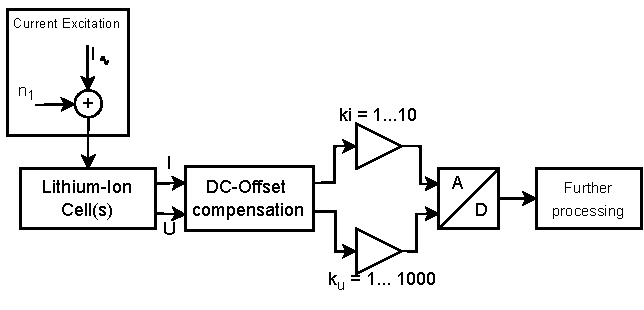
\includegraphics[width=1\columnwidth]{../img/signalfluss_eis.pdf}
	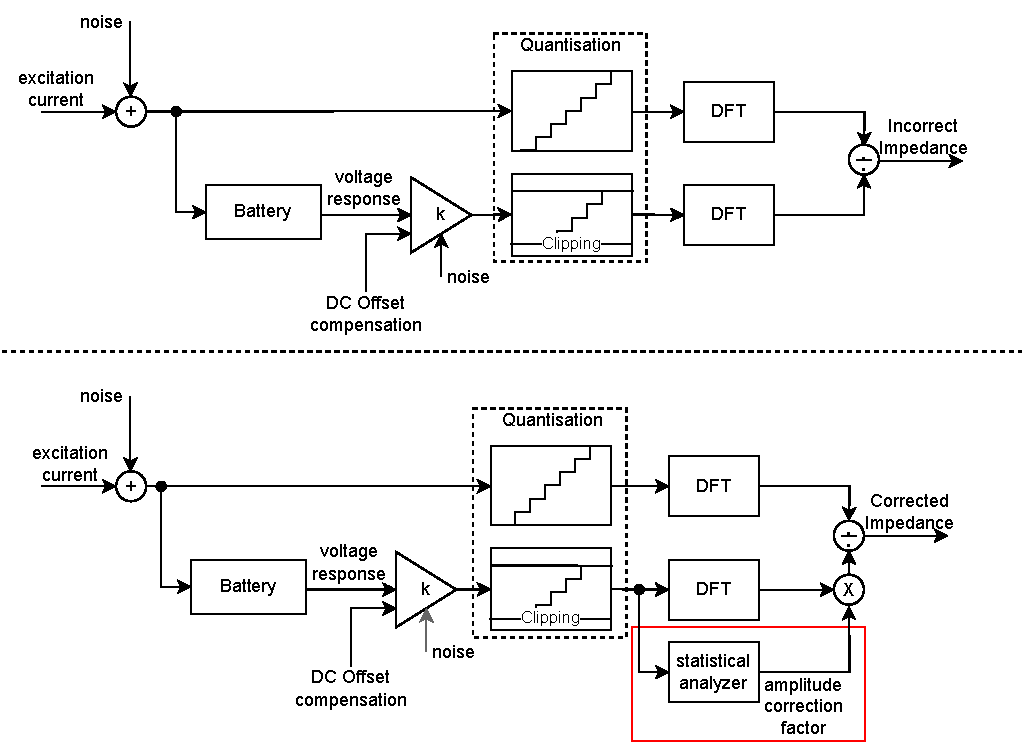
\includegraphics[width=1\textwidth]{../img/system.pdf}
	\caption{Die Berechnung der Impedanz wird infolge von unbekannter Amplitude und Rauscheinflüssen verfälscht, wenn eine Sättigung des ADC eintritt (oben). Zielstellung des vorgestellten Verfahrens ist die Verfälschung durch einen Amplitude-Korrekturfaktor weitgehend auszugleichen (unten).}
	\label{fig:system}
\end{figure*}
%\section{Problembeschreibung}    
%Eine besondere Herausforderung in dem gegebenen System ist das Erfassen der Spannungsantwort. Wie einleitend schon
%aufgeführt liegt die erwartete Amplitude der Spannungsantwort im niedrigen Millivolt Bereich. Dies führt zu einem erwartungsgemäß schlechtem Störabstand, da einerseits die Störungen der Anregung sich auf die Spannungsantwort übertragen und gleichzeitig das Signal nur knapp über Störungen wie dem Grundrauschen Rauschen des Systems liegen. Das Verstärken eines stark verrauschten Signals führt zu einer schlechten Ausnutzung des Dynamikbereichs des ADCs, da die Rauschanteile des Signals den ADC frühzeitig in Sättigung treiben. 

Die Abb.~\ref{fig:Rauschanteil} zeigt, dass schon durch Sättigung des ADC nur durch Rauschanteile des Signals die berechnete Amplitude verfälscht wird, obwohl das Signalamplitude ohne Rauschen noch nicht übersteuert ist. Ob sich der ADC in Sättigung befindet und in wie weit die Amplitude verfälscht ist, kann durch eine Klirrfaktoranalyse festgestellt werden. Sie ist jedoch vergleichsweise rechenaufwändig.  
Wenn sich die Ableitung des gemessenen Signals Abschnittsweise zu null ergibt, kann eine Aussage über den Grad der Übersteuerung getroffen werden. Bei starken Rauschanteilen ist diese Methode ungeeignet. Auch das einfache betrachten der Minimal- und Maximalwerten im ADC kann für eine Beurteilung des Sättigungszustands des ADC eingesetzt werden [6].
Weiterhin ist es für eine optimale Aussteuerung notwendig, dass sich die Abtastwerte des Signals möglichst symmetrisch im Dynamikbereich des ADC verteilen. Dies wird ebenfalls durch das Zusammenwirken von analoger und digitaler Signalverarbeitung sichergestellt. Das vorgestellte Verfahren lässt eine Auswertung der Symmetrie der blockweise erfassten Messwerte zu und steuert damit die erforderliche Referenzspannung, welche von der veränderlichen Batteriespannung subtrahiert wird. Diese Kompensierung muss hinreichend präzise erfolgen, da anschließend hohen Verstärkungsfaktoren verwendet werden. 

 \begin{figure}[h!] 
	\centering 
	%\includegraphics[width=.8\columnwidth]{PositionSensorArrayII_P-crop.pdf}
	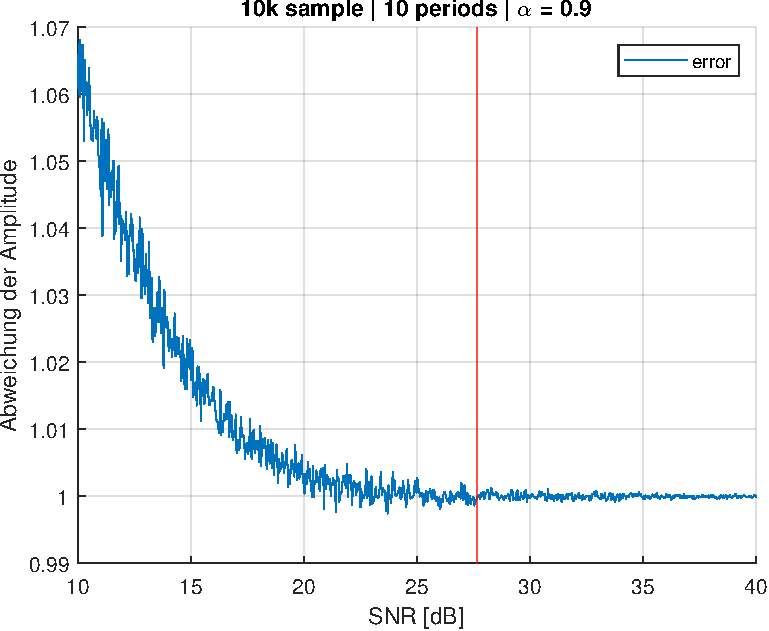
\includegraphics[width=.8\columnwidth]{../img/noise-err.pdf}
	\caption{Die Abweichung entsteht durch die Sättigung des ADC durch Rauschanteil. Dies wirkt sich in der DFT auf die Berechnung der Amplitude aus. Schon kleine Anteile des Rauschens in Sättigung führen zu einer rechnerischen Abweichung.}
	\label{fig:Rauschanteil}
\end{figure}

\section{Lösungsansatz} 

Der Lösungsansatz besteht in der stochastischen Auswertung der Verteilung der Datenpunkte des Signals. Mit den gemessenen Charakteristiken wird ein Rückschluss auf den Grad des Fehlers der Messung ermöglicht. Entsprechende Amplitude-Korrekturfaktoren können zur Korrektur angewandt werden. Das Histogramm wird in $h_b = 2^n$ mit $n = 12$ Klassen aufgeteilt, dies entspricht den Quantisierungsstufen des ADC. Die Ränder $h_0$ und $h_b$ beinhalten die Datenpunkte in den Grenzbereichen des Dynamikumfanges des ADC. Über den Anteil der Datenpunkte, welche sich in den Randbereichen befinden, lässt sich eine Aussage über den Sättigungsgrad des ADC treffen. In Kombination mit den stochastischen Momenten Varianz und Kurtosis kann der Fehler welcher, durch Sättigung des ADC entsteht, einem Amplitude-Korrekturfaktor zugeordnet und anschließend kompensiert werden.  

\subsection{Histogramme sinusförmiger Signale }
Das Histogramm im allgemeinen findet unter anderem Anwendung im Testen und der Charakterisierung von Analog-Digital-Wandlern. Es wird mittels sinusförmiger Signale und einer Auswertung via Histogramm ein Rückschluss auf die Qualität des ADC selbst gezogen [7]. Periodische sinusförmige Signale weisen eine charakteristische Verteilungsfunktion auf, welche qualitativ einem Spezialfall der Beta-Verteilung für $\alpha = \beta$ entspricht. In der Abb.~\ref{fig:Histogramm-Gain} (oben) ist die charakteristische Ausprägung des Histogramms eines periodengenauen, sinusförmigen Signals für steigende Verstärkungen zu sehen. Zu erkennen ist, dass die Datenpunkte sich bei zunehmender Verstärkung des Signals in die Randbereiche verlagern. Dies wird auch durch die Änderung der Varianz und Kurtosis der Verteilungen deutlich.
\begin{figure}[h!] 
	\centering 
	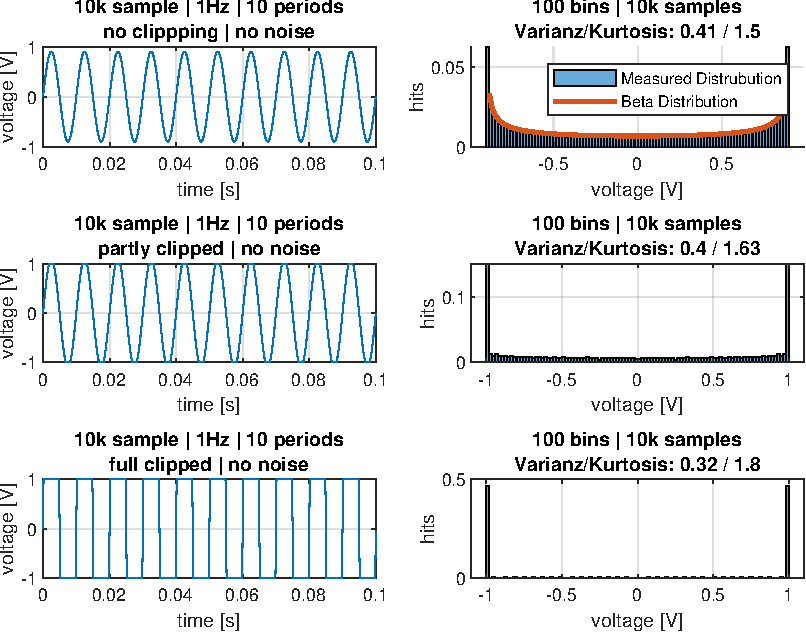
\includegraphics[width=.9\columnwidth]{../img/beta-distribution.pdf}
	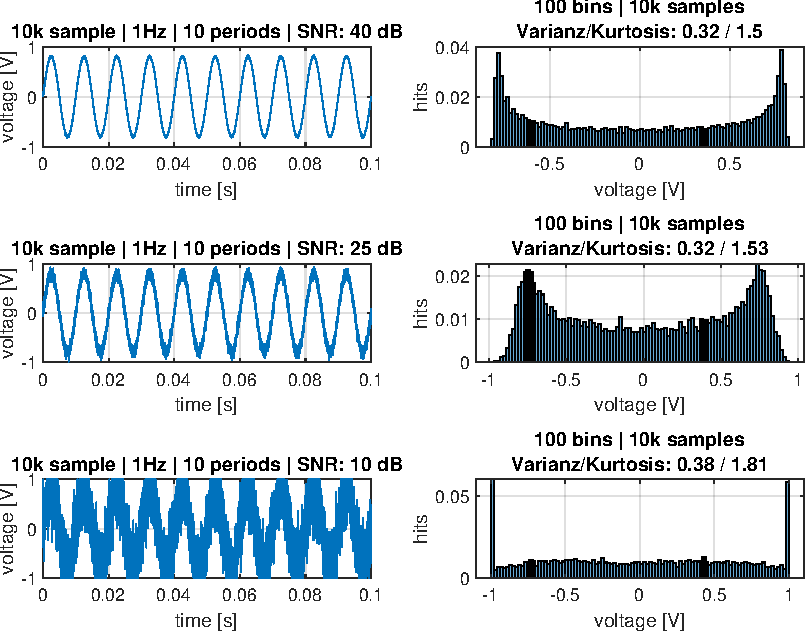
\includegraphics[width=.9\columnwidth]{../img/noise-histogramm.pdf}
	\caption{Die oberen drei Histogramme werden durch rauschfreie Signale mit verschiedener Amplitude erzeugt. Dabei werden unterschiedliche Sättigunggrade dargestellt. Die unteren drei Histogramme zeigen verschiedene Rauschverhältnisse bei konstanter Amplitude.}
	\label{fig:Histogramm-Gain}
\end{figure} 
Die Abb.~\ref{fig:Histogramm-Gain} (unten) zeigt den Verlauf des Histogramms bei zunehmendem Rauschen (Verschlechterung des SNR) und konstanter Verstärkung. Im Vergleich zu einem rauschfreien sinusförmigen Signalverlauf bildet sich das Histogramm weniger markant aus. Die Datenpunkte verteilen sich gleichförmiger über alle Klassen des Histogramms, bis die Sättigung durch starkes Rauschen wieder zu einer Fokussierung der Datenpunkte in den Randbereichen führt. Auffällig ist außerdem, dass die Varianz bis zur (Teil-)Sättigung des ADC wenig Veränderung aufweist, wohingegen die Kurtosis sensitiver reagiert. Diese Charakteristiken kann verwendet werden, um Rückschlüsse auf die Signalqualität des vorliegenden Signals zu ziehen. Ziel des Ansatzes ist es, eine recheneffiziente Methode zur Beurteilung der Signalqualität und ggf. der Korrektur des Signals zu erhalten. Die Beurteilung der Signalqualität muss anwendungsbezogen erfolgen. In der konkreten Anwendung der EIS-Sensorik ist das primäre Ziel eine maximale Auflösung des Signals, ohne die Berechnung der Amplitude des Signals durch Sättigung des ADC zu verfälschen. Es ist demnach wünschenswert, den Dynamikbereich voll auszusteuern und eine gewisse Sättigung zuzulassen, solange eine Korrektur möglich ist.

\section{Ermittlung der Korrekturfaktoren}
Der Zusammenhang der Korrekturfaktoren wird über den Störabstand und der Verstärkung des Signals mit den drei angeführten Größen: 
\begin{itemize}
	\item Anteil der Datenpunkte in Sättigung %Gl.~\ref{eq:dist_sat}, Kurtosis %aus Gl.~\ref{eq:kurtosis} 
	\item Varianz der Häufigkeitsverteilung Signals (bereinigt\footnote[1]{Das Signal beinhaltet keine Datenpunkte, welche sich im Sättigungsbereich des ADC befinden.\label{foot:bereinigt}})
	\item Kurtosis der Häufigkeitsverteilung des Signals (bereinigt\footref{foot:bereinigt})
\end{itemize}

%und Varianz %aus Gl.~\ref{eq:varianz} 
%aus der Häufigkeitsverteilung des Signals.

Der Anteil der Datenpunkte in Sättigung ergibt sich aus der Anzahl der Datenpunkte in den äußersten Klassen des Histogramms nach Gl.~\eqref{eq:dist_sat}. Der Dynamikbereich des ADC wird bei 12-Bit in $b=4096$ Stufen aufgelöst. Jeder Datenpunkt kann in einem Histogramm einer Klasse $b$ zugeordnet werden. Was der Verteilung des Signals entspricht. 

\begin{equation}
	\label{eq:dist_sat}
	h_{sat} = h_0 + h_b = \frac{n_0 + n_b}{n} \cdot 100
\end{equation}

Die Ermittlung der Faktoren muss zuvor mittels Simulation experimentell erfolgen. In der Simulation wird ein ideales Referenzsignal $u_{Ref}(t)$ verwendet. Für die Berechnung eines Korrekturfaktors wird nur die Amplitude der Grundfrequenz $f_0$ im Spektrum betrachtet. Mit Hilfe der Fourier Analyse ergibt sich die Referenzamplitude $\hat{U}_{Ref}(f_0)$. Für die Berechnung einer Korrekturfaktoren $K$ ist es notwendig, für relevanten Kombinationen aus SNR $n$ und Verstärkung $g$ jeweils die Amplitude $\hat{U}_{n,g}(f_0)$ der Grundfrequenz $f_0$ der Signale $u_{n,g}(t)$, die bereinigte\footref{foot:bereinigt} Kurtosis $w(u_{n,g}(t))$ und die Varianz $\sigma^2(u_{n,g}(t))$ zu berechnen sowie den Sättigungsgrad des ADC $h_{sat}(u_{n,g}(t))$ zu bestimmen. Die Signale werden zur Ermittlung der Korrekturfaktoren mit additivem Rauschen beaufschlagt, multiplikativ verstärkt in den Minimal- und Maximalwerten begrenzt und Quantifiziert. Anschließend werden Verstärkung und SNR auf die stochastischen Größen des Signals abgebildet. Die Abbildung ermöglicht den umgekehrten Zugriff anhand der stochastischen Größen der späteren Messung auf die Amplitude-Korrekturfaktoren.
Für einen Korrekturfaktor ergibt sich Gl.~\eqref{eq:corr}.

\begin{equation}
	\label{eq:corr}
	k_{n,g} = \frac{|\hat{U}_{Ref}(f_0)|}{|\hat{U}_{n,g}(f_0)|} % = \frac{|\mathcal{F}(u_{Ref}(t))(f_0)|}{|\mathcal{F}(u_{n,g}(t))(f_0)|}
\end{equation}

Die Abb.~\ref{fig:lut} zeigt die Charakteristik der stochastischen Momente (bereinigt\footref{foot:bereinigt} ) und den Sättigungsgrad für die Signale $u_{n,g}(t)$. 
Der Amplitude-Korrekturfaktor wird den stochastischen Momenten und dem Sättigungsgrad $h_{sat}$ zugeordnet. Zunächst wird Kalibrationsphase durchgeführt, in welcher eine Zuordnung des Amplituden-Korrekturfaktors anhand der stochastischen Eigenschaften des Ausgangssignals erfolgt. Diese Zuordnung wird als tabellarische Abbildung in einer Look-Up Tabelle (LUT) gespeichert, siehe Abb.~\ref{fig:factor_eval}. 
Die Einträge der LUT werden durch Simualtionsläufe für die Kombinationen der Parameter Verstärkung und Rauschanteil erzeugt. Dabei durchlaufen die Parameter stufenweise Bereiche, die für die Anwendung zuvor abgeschätzt wurden. Sofern dabei Einträge der LUT nicht besetzt werden, erfolgt eine Interpolation. %, hierzu eignet sich die MATLAB-Funktion griddata. 
Die Mehrfachbesetzung von Einträgen in der LUT kam in der Simulation selten vor, in diesem Fall wurde der vorherige Eintrag überschrieben. Der resultierende Fehler hat einen vernachlässigbaren Einfluss. Dies entspricht auch der geringen Abweichung in der Differenzdarstellung in Abb.~\ref{fig:lut} (unten rechts). In der späteren Nutzungsphase kann das Messsignal nach den stochastischen Eigenschaften blockweise analysiert werden. Die drei Ergebnisse der Analyse können unmittelbar als Index der LUT verwendet werden. Damit kann der Amplitude-Korrekturfaktor unmittelbar aus der LUT ausgelesen werden.
\begin{figure*}[th!]
	\centering
	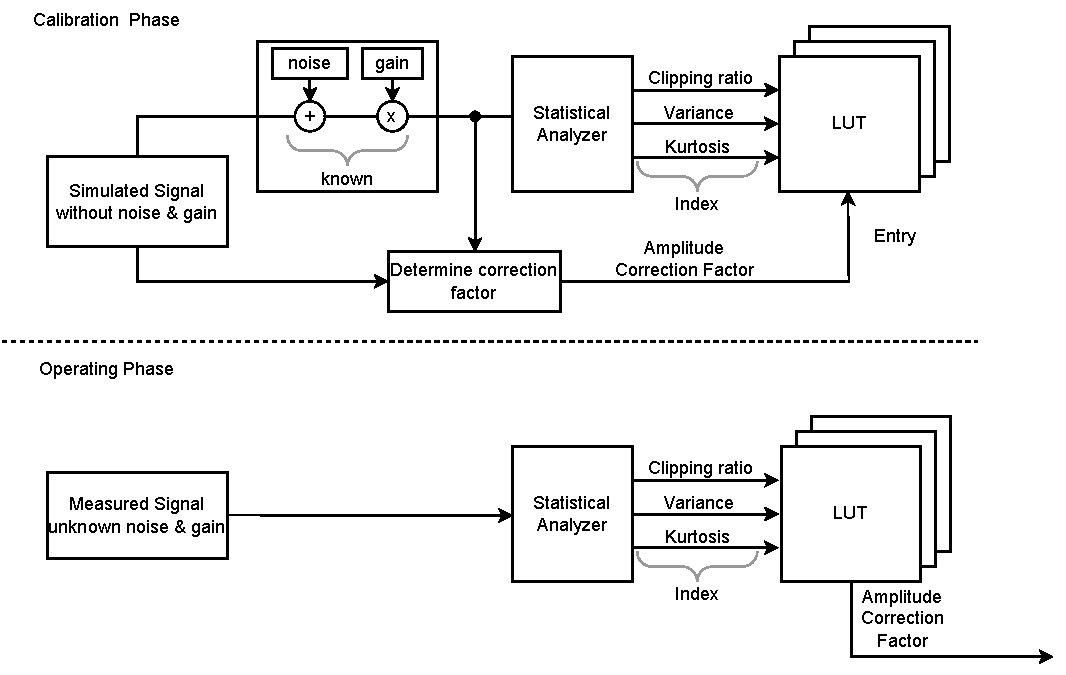
\includegraphics[width=.9\textwidth]{../img/factor.pdf}
	\caption{Während der Kalibrationsphase wird die LUT erstellt. Während der Messung liefert die LUT den Amplituden-Korrekturfaktor.}
	\label{fig:factor_eval} 
\end{figure*}
Die Abb.~\ref{fig:lut} (oben) zeigt die stochastischen Eigenschaften über Verstärkung und SNR der Signale. Die Merkmale weisen eine Sensitivität in verschiedenen Bereichen von Verstärkung und Rauschverhalten auf. Zur weiteren Optimierung kann der Korrekturfaktor auch komplex bestimmt werden, der aktuelle Ansatz verwendet den Betrag und skaliert den Imaginär- und Realteil der komplexen Amplitude. Eine Alternative Möglichkeit ist ein Funktionsfit mit min. drei gewichteten Koeffizienten. Erste Untersuchungen zeigten vergleichbare Ergebnisse.


%ation\footnote[2]{Der Quellcode zur Simulation: https://github.com/TobiasFrahm/histogramm-verfahren} wird die Korrekturfaktormatrix berechnet und überprüft, ob mit den ermittelten Faktoren eine Korrektur der Amplitude möglich ist. 
%ete Batteriemodell zur Berechnung der Spannungsantwort ist ein RRC-Modell ($R0 = \SI{6}{m\Omega}, R1=\SI{4}{m\Omega}, C1=\SI{500}{mF}$). Die Anregung erfolgt mit einer Amplitude von $\SI{1}{A}$, der erwartete Wechselanteil der Spannungsantwort liegt bei ca. $\SI{10}{mV}$. Die Spannungsantwort wird transient berechnet. Der durch die Batteriespannung aufgeschlagene Gleichanteil der Spannungsantwort wird Subtrahiert. Je nach angewandtem Messverfahren, ist dies auch für die Strommessung notwendig. Die Quantisierung erfolgt mit einem Dynamikbereich von $12$-Bit über $\SI{3.3}{V}$, die Sättigung des ADC wird durch limitieren der Werte simuliert. Die Grenzwerte liegen für das Minimum bei $\SI{0}{V}$ und im Maxima bei $\SI{3.3}{V}$. Die Verarbeitung der Signale erfolgt blockweise. Für die Bildung der Referenzfaktoren, wird die Simulation und Berechnung für den gesamten anwendungsbezogen Wertebereich der Verstärkung und dem Störabstand durchgeführt. In der späteren Anwendung wird auf die berechnete Korrekturfaktormatrix über die stochastischen Momente und dem Anteil der Datenpunkte in Sättigung zu gegriffen. Der entnommene Korrekturfaktor wird multiplikativ mit der komplexen Amplitude im Frequenzbereich verrechnet, Gl.~\eqref{eq:corr_mat}. Die Matrix wird durch den vollständigen Parametervarianz der Signalamplitude und des additiven Rauschens durchgeführt. Für jeden Schritt des parameterlaufs werden die Größen Sättigungsgrad, Varianz und Kurtosis errechnet. Aus diese Größen wird jeweils ein Indextripel gebildet.
%
%Der Statistical Analyzer (SA) aus Abb.~\ref{fig:Simulation} wird in Abb.~\ref{fig:sa} näher beschrieben. Der SA wertet die Verteilung des Signals mittels der stochastischen Methoden aus. Aus der Verteilung können neben der Bestimmung der Maße für die Amplitudenkorrektur weitere Signaleigenschaften, wie die Lage des Signals im ADC und den Grad der Aussteuerung des ADC abgeleitet werde. Für die Kompensierung des Gleichanteils kann mittels der Schiefe und der Nulllage ermittelt werden, ob das Signal den ADC über- oder  untersteuert. Diese Eigenschaften können beispielsweise für eine Lage- oder Verstärkungsregelung verwendet werden [5].

\begin{figure*}[th!]
	\centering
	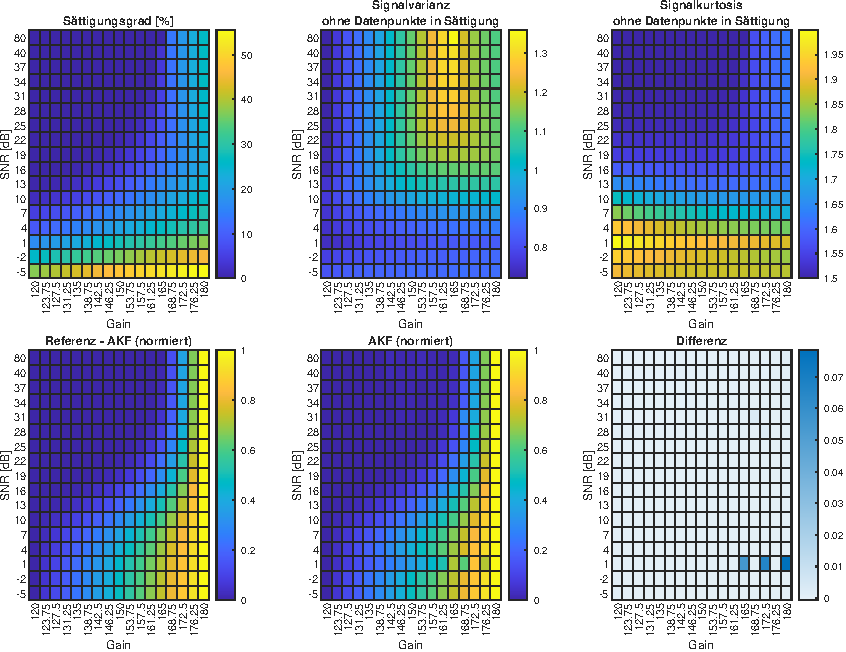
\includegraphics[width=.9\textwidth]{../img/lut.pdf}
	\caption{Die stochastischen Merkmale der Verteilung (oben) werden Verwendet, um auf die Signalqualität zu schließen. Die Korrekturfaktoren (unten) werden für jede Kombination von Verstärkungsfaktoren und Rauschabstand gebildet des Signals gebildet.}
	\label{fig:lut} 
\end{figure*}


\section{Simulation}

Zunächst werden die Amplituden-Korrekturfaktoren in der Simulation\footnote[2]{Der Quellcode zur Simulation: https://github.com/TobiasFrahm/histogramm-verfahren} berechnet. Hierfür wurde der in Abb.~\ref{fig:factor_eval} gezeigt Signalfluss implementiert. Das Stromsignal wird vor der Berechnung der Spannungsantwort mit additivem, weißem Rauschen beaufschlagt. Das verwendete Batteriemodell zur Berechnung der Spannungsantwort ist ein RRC-Modell ($R0 = \SI{6}{m\Omega}, R1=\SI{4}{m\Omega}, C1=\SI{500}{mF}$). Die Rauscheinfluss am Verstärker wurden in der Simulation vernachlässigt. Die Anregung erfolgt mit einer Amplitude von $\SI{1}{A}$, der erwartete Wechselanteil der Spannungsantwort liegt bei ca. $\SI{10}{mV}$. Die Spannungsantwort wird transient berechnet. Der durch die Batteriespannung aufgeschlagene Gleichanteil der Spannungsantwort wird Subtrahiert. Je nach angewandtem Messverfahren, ist dies auch für die Strommessung notwendig. Die Quantisierung erfolgt mit einem Dynamikbereich von $12$-Bit über $\SI{3.3}{V}$, die Sättigung des ADC wird durch limitieren der Werte simuliert. Die Grenzwerte liegen für das Minimum bei $\SI{0}{V}$ und im Maxima bei $\SI{3.3}{V}$. Die Verarbeitung der Signale erfolgt blockweise. Für die Bildung der Referenzfaktoren, wird die Simulation und Berechnung für den gesamten anwendungsbezogen Wertebereich der Verstärkung und dem Störabstand durchgeführt. In der späteren Anwendung wird auf die berechnete Korrekturfaktormatrix über die stochastischen Momente und dem Anteil der Datenpunkte in Sättigung zu gegriffen. Der entnommene Korrekturfaktor wird multiplikativ mit der komplexen Amplitude im Frequenzbereich verrechnet, Gl.~\eqref{eq:corr_mat}. Die Matrix wird durch den vollständigen Parametervarianz der Signalamplitude und des additiven Rauschens durchgeführt. Für jeden Schritt des parameterlaufs werden die Größen Sättigungsgrad, Varianz und Kurtosis errechnet. Aus diese Größen wird jeweils ein Indextripel gebildet.

\begin{equation}
	\label{eq:corr_mat}
	Z_k(f) = \frac{\hat{U}_{n,g}(f) \cdot k_{v,k,c}^{n,g}}{\hat{I}(f)}
\end{equation}	

(SA) aus Abb.~\ref{fig:factor_eval} wertet die Verteilung des Signals mittels der stochastischen Methoden aus. Aus der Verteilung können neben der Bestimmung der Maße für die Amplitudenkorrektur weitere Signaleigenschaften, wie die Lage des Signals im ADC und den Grad der Aussteuerung des ADC abgeleitet werde. Für die Kompensierung des Gleichanteils kann mittels der Schiefe und der Nulllage ermittelt werden, ob das Signal den ADC über- oder  untersteuert. Diese Eigenschaften können beispielsweise für eine Lage- oder Verstärkungsregelung verwendet werden [5].


\section{Ergebnisse und Diskussion}
Die Ergebnisse in Abb.~\ref{fig:Ergebnisse} zeigen eine deutliche Verbesserung in der Berechnung der EIS. Die Berechnung der EIS weist insbesondere in den niederfrequenten Bereichen einen ausgeprägten Fehler auf. Hier ist ein Zusammenhang mit dem Frequenzgang des verwendeten Modells zu vermuten. Die mit steigender Frequenz abnehmende Amplitude führt zu weniger Signalsättigung und damit auch zu weniger Abweichung in der Messung. Hier kann anwendungsbezogen ein Schwellwert festgelegt werden, ab welchem eine Korrektur der Messung Sinn hat. Als Maß für einen Schwellwert bietet sich der Anteil der Datenpunkte in Sättigung an. Ein Vergleich mit den stochastischen Momenten aus Abb.~\ref{fig:lut} und dem root mean square error (RMSE) des Signals zeigt einen deutlichen Zusammenhang zwischen der Sättigung des Signals und der Varianz des Signals. Die Varianz reagiert bei einem guten Störabstand besonders sensitiv auf den Grad der Sättigung des Signals. Wie der Abb.~\ref{fig:Ergebnisse} in der Darstellung unten links zu entnehmen ist, wird der ADC durch das Signal bei einer Verstärkung von ca. $165$ in Sättigung getrieben. Dieser Bereich ist auch deutlich in der Varianz zu erkennen. Die Kurtosis weist bei geringer Verstärkung und gutem Störabstand hingegen weniger Änderung auf. Bei besonders schlechtem Störabstand ist kaum noch eine Änderung zu erkennen. Der sensitive Bereich liegt bei der Kurtosis zwischen $22dB - 1dB$ und oberhalb des Sättigungsbereichs bei einem Verstärkungsfaktor von ca. $160$. Die Kombination stochastischen Größe ergeben ein gutes Maß zur Klassifizierung des Signals. Die Differenz zwischen $K_{n,g}$ und $K_{v,k,c}$ (Abb.~\ref{fig:lut}, unten rechts) ist gering und zeigt nur geringe Abweichungen. Die Ergebnisse der Berechnung zeigen dahingegen über das gesamte Spektrum bei großer Abweichung eine deutliche Verbesserung der Berechnung.
\begin{figure*}[hbt!]
	\centering
	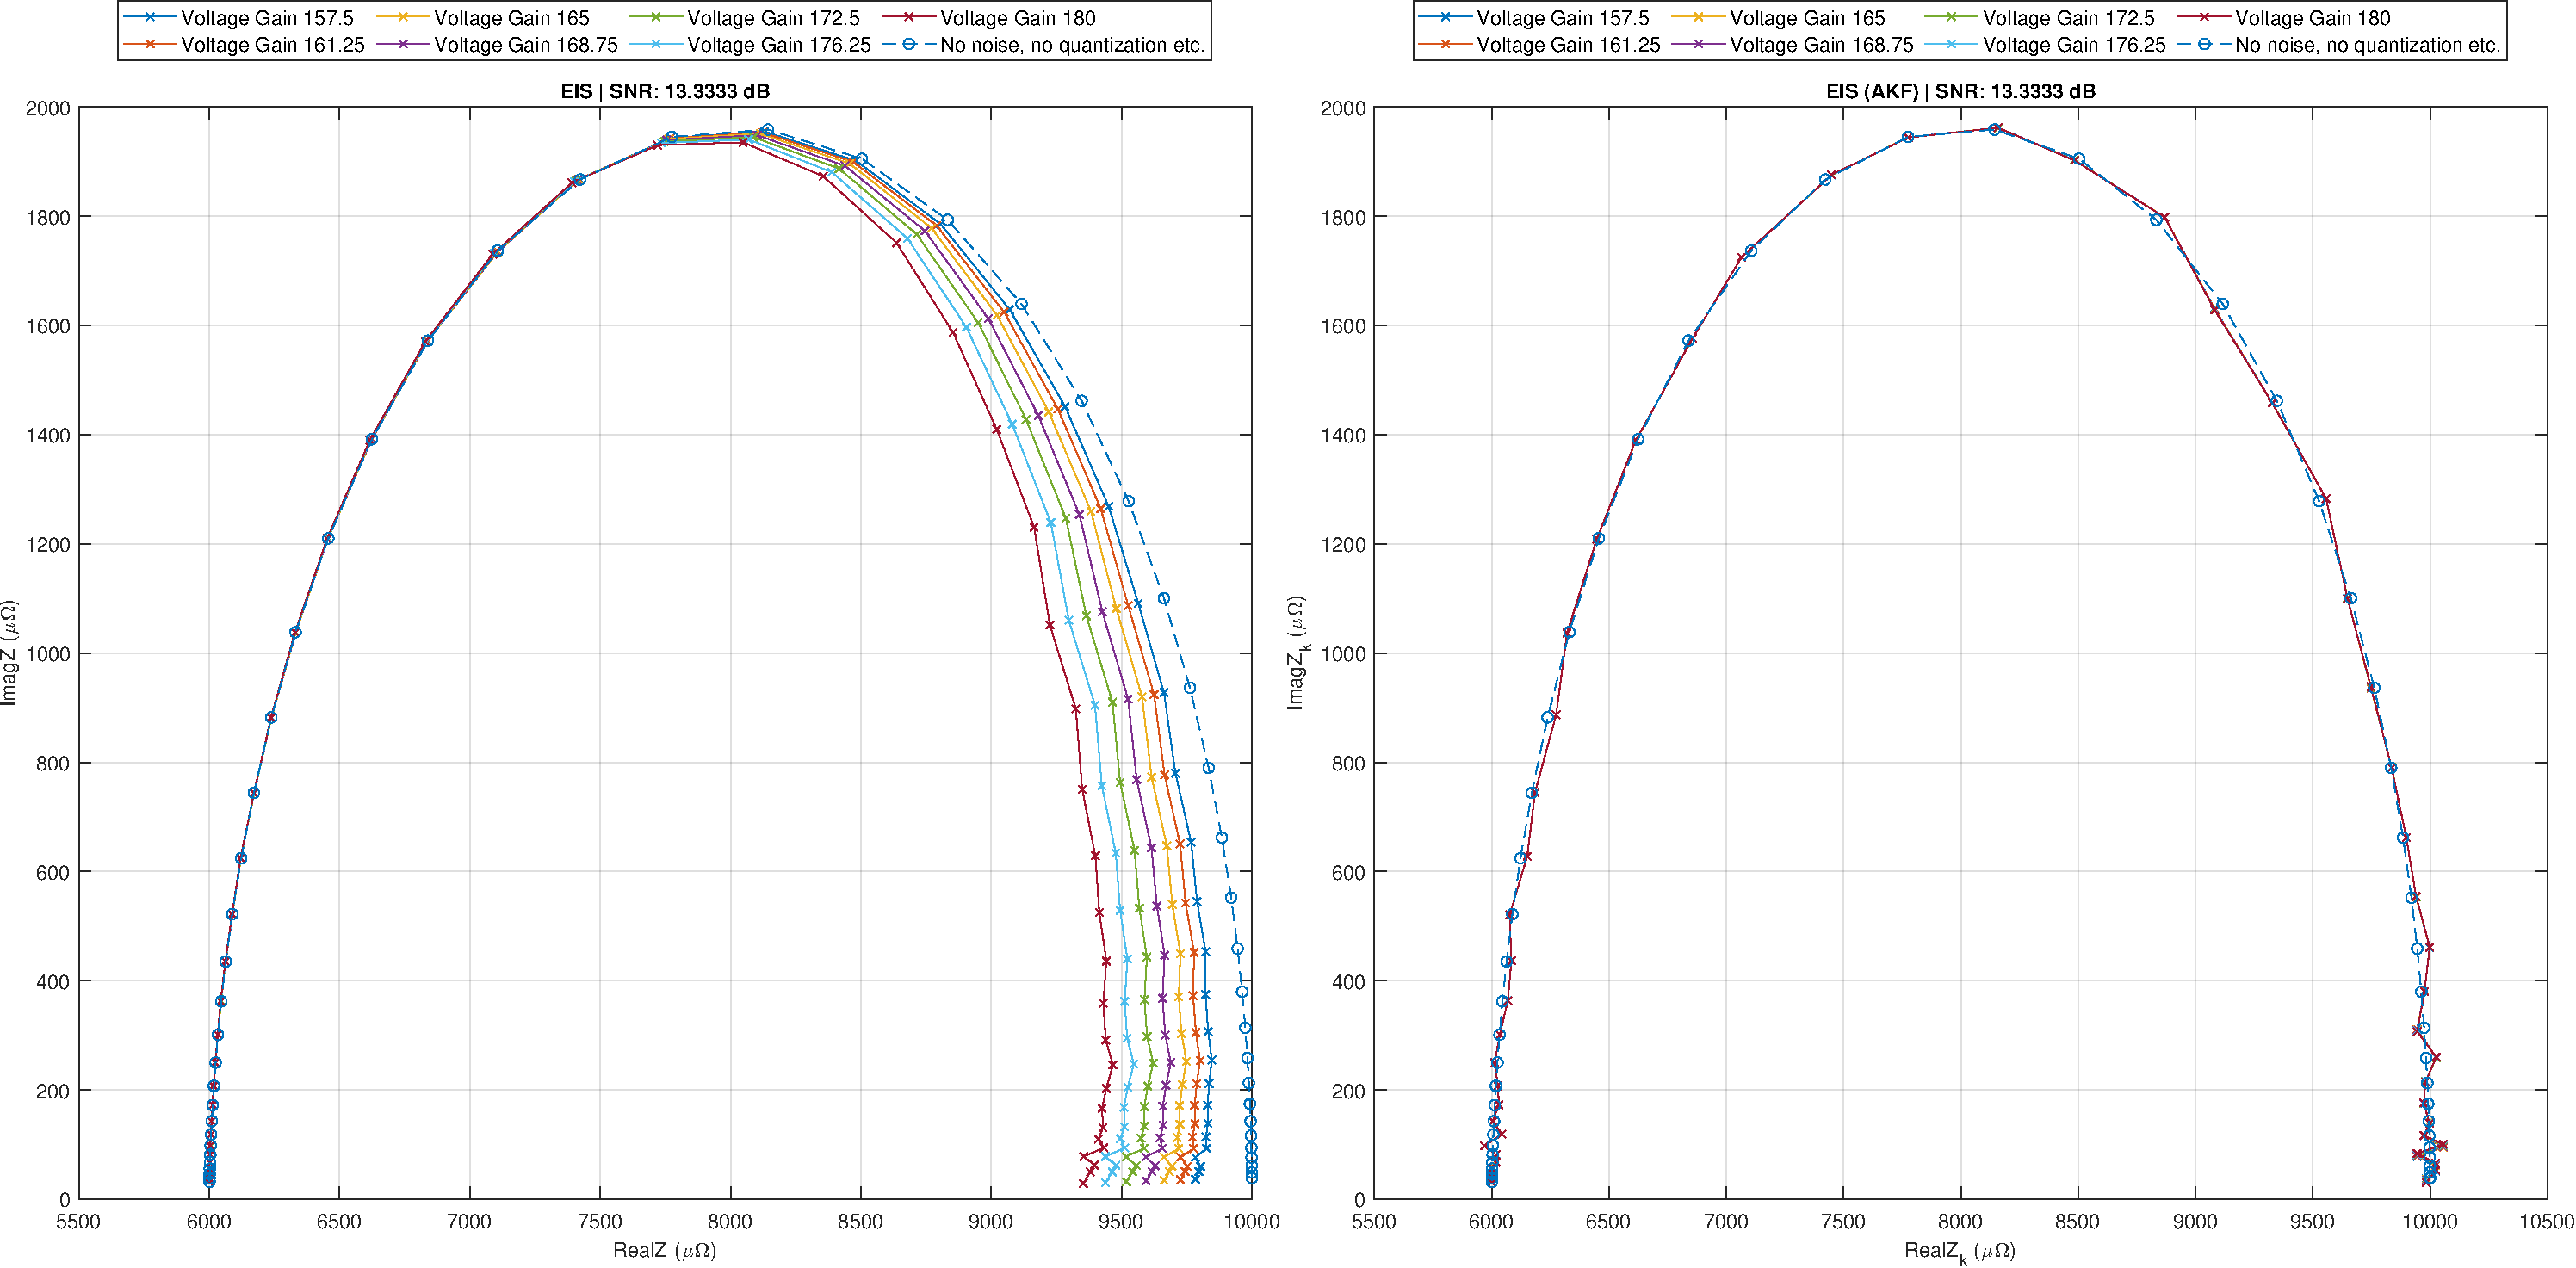
\includegraphics[width=.99\textwidth]{../img/ergebnisse.pdf}
	\caption{Das EIS-Spektrum weist nach der Korrektur eine deutliche Verbesserung im direkten Vergleich auf. Die Korrektur ist besonders bei hohen Verstärkungen wirksam, was auf den Amplitudengang des Batteriemodells zurückzuführen ist.}
	\label{fig:Ergebnisse} 
\end{figure*}
   
%\renewcommand*{\bibfont}{\fontsize{9pt}{10pt}\selectfont}
%\selectlanguage{ngerman} 
%\selectbiblanguage{ngerman}

%\printbibliography[title=Literaturnachweis] 
\begin{thebibliography}{[99]}
	\bibitem{Chan-2012}
	A. D. C. Chan. J. R. Green. D.Maclsaac. G. D. Fraser, „Detection of ADC clipping, quantization noise, and amplifier saturation in surface electromyography,“ IEEE International Symposium on Medical Measurements and Applications Proceedings, 2012.
	
	\bibitem{Jung-1993}
	P. Jung, „Periodically driven stochastic systems”, Physics Reports,  pp. 175-295, 1993.
	
	\bibitem{Roscher-2016}
	V. Roscher. K.-R. Riemschneider. N. Sassano, „Batterie-Zellensensoren mit drahtloser Kommunikation und verteilter Signalverarbeitung,“ in Automobil-Sensorik, T. Tille, Hrsg., Springer, 2016.
	
	\bibitem{Hammerschmidt-2023}
	T. Hammerschmidt, J.P. Schmidt, „Impedanzsensorik für Batteriezellen in Elektro-Fahrzeugen,“ in Automobil-Sensorik, T. Tille, Hrsg., Springer, 2016.
	
	\bibitem{Frahm-2023}
	T. Frahm „Sensorsystem für die Impedanzspektroskopie in Fahrzeugbatterien: Analogvorstufe, Signalverarbeitung und Software“, Masterarbeit, HAW Hamburg, 2023.
	
	\bibitem{Fraser-2012}
	G. D. Fraser, A. D. C. Chan, J. R. Green and D. MacIsaac, "Detection of ADC clipping, quantization noise, and amplifier saturation in surface electromyography," 2012 IEEE International Symposium on Medical Measurements and Applications Proceedings, Budapest, Hungary, 2012, pp. 1-5, doi: 10.1109/MeMeA.2012.6226629.
	
	\bibitem{Gamad-2009}
	R.S. Gamad, D.K. Mishra,
	Gain error, offset error and ENOB estimation of an A/D converter using histogram technique,
	Measurement,
	Volume 42, Issue 4,
	2009,
	Pages 570-576,
	ISSN 0263-2241,
	https://doi.org/10.1016/j.measurement.2008.10.003.
	
	\bibitem{Abel-1991}
	J. S. Abel and J. O. Smith, III, “Restoring a clipped signal,” in
	Proc. IEEE ICASSP, Toronto, Ontario, Canada, Apr 1991, pp.
	1745–1748.	

	\bibitem{Ting-2013}
	S. -K. Ting and A. H. Sayed, "Mitigation of clipping in sensors," 2013 IEEE International Conference on Acoustics, Speech and Signal Processing, Vancouver, BC, Canada, 2013, pp. 5934-5938, doi: 10.1109/ICASSP.2013.6638803.

%	\bibitem{Zhou-2019}
%	N. Zhou, J. Wang, B. Sun, R. Liu and N. Hu, "The Automatic Repairing Method Addressing Clipping Distortions and Frictional Noises in Electronic Stethoscope," 2019 IEEE 7th International Conference on Bioinformatics and Computational Biology ( ICBCB), Hangzhou, China, 2019, pp. 195-199, doi: 10.1109/ICBCB.2019.8854669.

	
\end{thebibliography}
	

 
\end{document} 